\documentclass[10pt]{beamer}
\usepackage[utf8]{inputenc}
\usetheme{Hannover}
\usefonttheme{serif}
\newcommand{\scriptword}[1]{\textsf{\ttfamily #1}}
\newcommand{\fig}[1]{Fig. \ref{#1}} % Definitions for Figure-References
\setbeamerfont{frametitle}{size=\large}
\usepackage{makecell}
\usepackage{bigstrut}

\setbeamertemplate{navigation symbols}{}

\usepackage{filecontents}
\begin{filecontents}{\jobname.bib}
@article{Park,
	author = {Park, C.},
	title = {Review of chemical-kinetic problems of future {NASA} missions,
		{I}: {E}arth entries},
	journal = {Journal of Thermophysics and Heat Transfer},
	volume = {7},
	number = {3},
	year = {1993}}

@article{Shatalov,
	author = {Ibraguimova, L. B. and Sergievskaya, A. L. and Levashov, V. Yu. and Shatalov, O. P. and Tunik, Yu. V. and Zabelinskii, I. E.},
	title = {Investigation of oxygen dissociation and vibrational relaxation
		at temperatures 4000-10800 {K}},
	journal = {The Journal of Chemical Physics},
	volume = {139},
	number = {3},
	year = {2013}}
\end{filecontents}

\usepackage[style=verbose,backend=biber]{biblatex}
\addbibresource{\jobname.bib}


\title{2-D Hypersonic Baffle Problem \\with \textit{hy2Foam}}
\author{Ivan Zanardi}
\institute{Politecnico di Milano}
\date{\today}

\AtBeginSection[]{
  \begin{frame}
    \frametitle{Outline}
    \tableofcontents[currentsection]
  \end{frame}
}


\begin{document}

\begin{frame}
  \titlepage
\end{frame}

\begin{frame}
  \frametitle{Outline} \tableofcontents
\end{frame}


\section{Hypersonic Flows}

\begin{frame}
  \frametitle{Introduction} Handling hypersonic flows means to deal with a
  multi-species, high-temperature, chemically reacting mixture of thermally
  perfect gases in high-speed flow, involving nonequilibrium chemical and
  thermal relaxation, radiation, ionization and
  ma\-gn\-eto\-hy\-dro\-dy\-na\-mic phenomena both in the continuum and
  rarefied flow regimes along flight trajectories of the relevant space
  vehicles.
\end{frame}

\begin{frame}
  \frametitle{Important Numbers} The re-entry vehicle flight trajectories
  traverse a wide range of Mach, Knudsen and Reynolds numbers, which are given
  by the following simple relations
  \begin{equation*}
    Ma=\frac{v}{a}\quad,\qquad Kn=\frac{\lambda}{L_{ref}}\quad,\qquad
    Re=\frac{\rho vL_{ref}}{\mu}\quad.
  \end{equation*}
  Thus, the vehicle experiences flow regimes going from subsonic to
  hypersonic, continuum to free-molecular, and laminar to turbulent.
\end{frame}

\begin{frame}
  \frametitle{Knudsen number} The Knudsen number is commonly employed to gauge
  the degree of gas rarefaction.
  \begin{figure}[ht]
    \centering 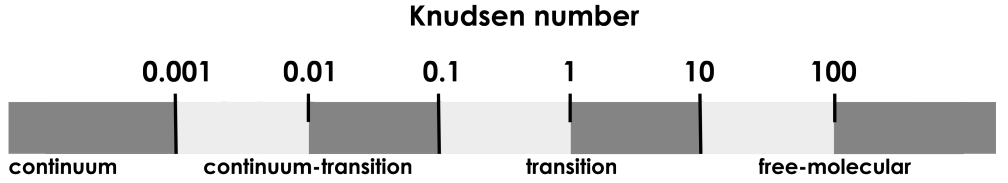
\includegraphics[width=0.8\textwidth]{./figures/knudsen.png}
    \caption{Flow regimes depending on the Knudsen number}
    \label{fig:Knudsen}
  \end{figure}
  In this study, exclusively the continuum regime is considered, so only
  flight trajectories under 90 km altitude in laminar flow condition are taken
  into account with $Kn<0.005$.
\end{frame}


\section{Problem description}

\begin{frame}
  The various contributions for hypersonic flow modeling have been considered
  with increasing complexity, in order to make a comparison between the
  different modelizations.
  \begin{table}[ht]
    \centering \footnotesize
    \caption{Simulations performed}
    \label{tab:simulations}
    \renewcommand{\arraystretch}{1.2} \setlength{\tabcolsep}{5pt}
    \begin{tabular}{ *{6}{c} }
      \noalign{\hrule height 1pt} \textbf{\makecell{Test\\Case}} &
      \textbf{\makecell{Eq. or\\Noneq.}}  &
      \textbf{\makecell{Vibro-elec.\\mode}}&\textbf{\makecell{V-T\\transfer}}
      & \textbf{\makecell{Chemistry\\ rates}}&\textbf{\makecell{C-V\\model}}
      \bigstrut \\ \hline C$_1$ & Eq. & Frozen & none & NR & NR \\ C$_2$ &
      Eq. & Active & none & NR & NR \\ C$_3$ & Eq. & Active & none & Park &
      none \\ C$_4$ & Noneq. & Active & Shatalov & NR & NR \\ C$_5$ & Noneq. &
      Active & Shatalov & Shatalov & Shatalov \\ \noalign{\hrule height 1pt}
    \end{tabular}
  \end{table}
\end{frame}

\begin{frame}
  The two chemical reactions considered in test case C$_3$ and C$_5$ are the
  irreversible mo\-le\-cu\-le-mo\-le\-cu\-le and mo\-le\-cu\-le-a\-tom
  dissociation of oxygen
  \begin{align*}
    & \mathrm{O}_2+\mathrm{O}_2 \longrightarrow \mathrm{O}_2+2\mathrm{O} \\ &
    \mathrm{O}_2+\mathrm{O}\phantom{_2} \longrightarrow 3\mathrm{O}
  \end{align*}
  The rate coefficients for the Shatalov's thermal nonequilibrium chemistry
  model are described in (\footcite{Shatalov}), while Park’s rates are shown
  in (\footcite{Park}).
\end{frame}


\begin{frame}
  The free-stream flow condition for the inlet patch are listed.
  \begin{table}[ht]
    \centering \footnotesize
    \caption{Free-stream flow condition}
    \label{tab:boundaryValues}
    \renewcommand{\arraystretch}{1.2} \setlength{\tabcolsep}{10pt}
    \begin{tabular}{ l l }
      \noalign{\hrule height 1pt} \textbf{Quantity} & \textbf{Value} \bigstrut
      \\ \hline Free-stream velocity, $u_\infty$ & 4440 m/s \\ Free-stream
      pressure, $p_\infty$ & 0.75 Pa \\ Free-stream temperature, $T_\infty$ &
      295 K \\ Free-stream Mach number, $Ma_\infty$ & 13.554 \\ Free-stream
      density, $\rho_\infty$ & 9.78449$\times$10$^{-6}$ kg/m$^3$
      \\ Free-stream number density, $n_\infty$ & 1.84143$\times$10$^{20}$
      m$^{-3}$ \\ Overall Knudsen number, $Kn_{ov}$ & 3.68944$\times$10$^{-3}$
      \\ \noalign{\hrule height 1pt}
    \end{tabular}
  \end{table}
\end{frame}


\section{Flow structure}

\begin{frame}
  \begin{figure}[ht]
    \centering 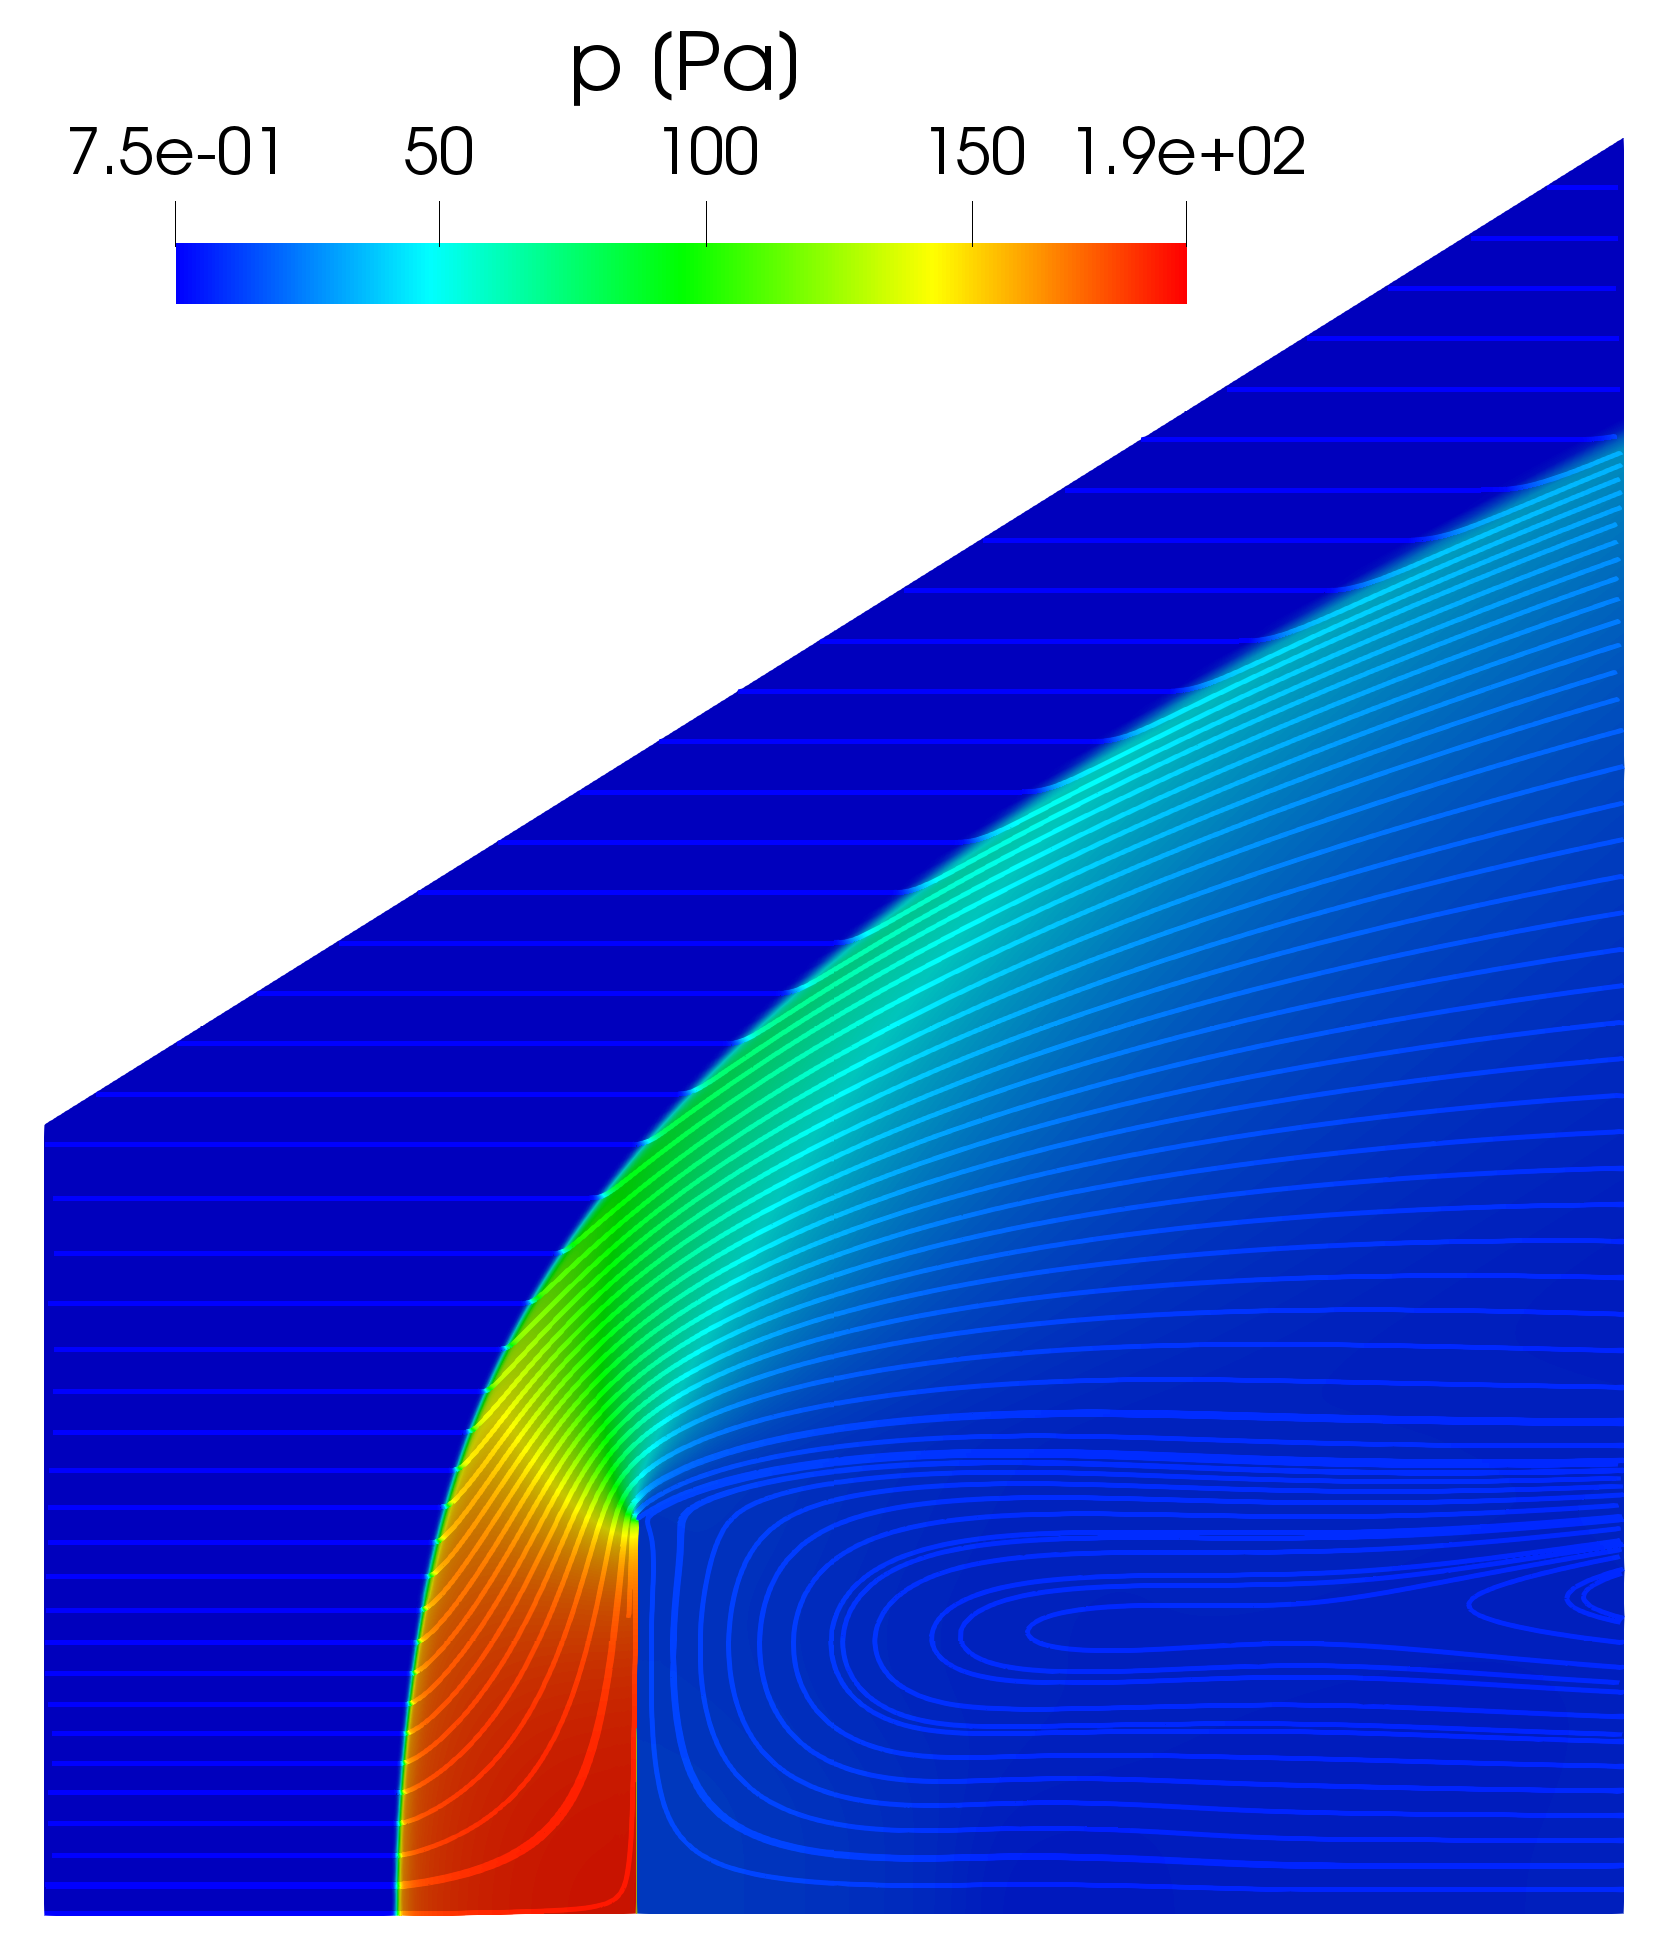
\includegraphics[width=0.6\textwidth]{./figures/flow.png}
    \caption{Test case 5}
  \end{figure}
\end{frame}


\section{Stagnation Line Quantities}

\begin{frame}
  In this section fundamental variables are analyzed along the stagnation line
  in front of the baffle body.
  \begin{figure}[ht]
    \centering 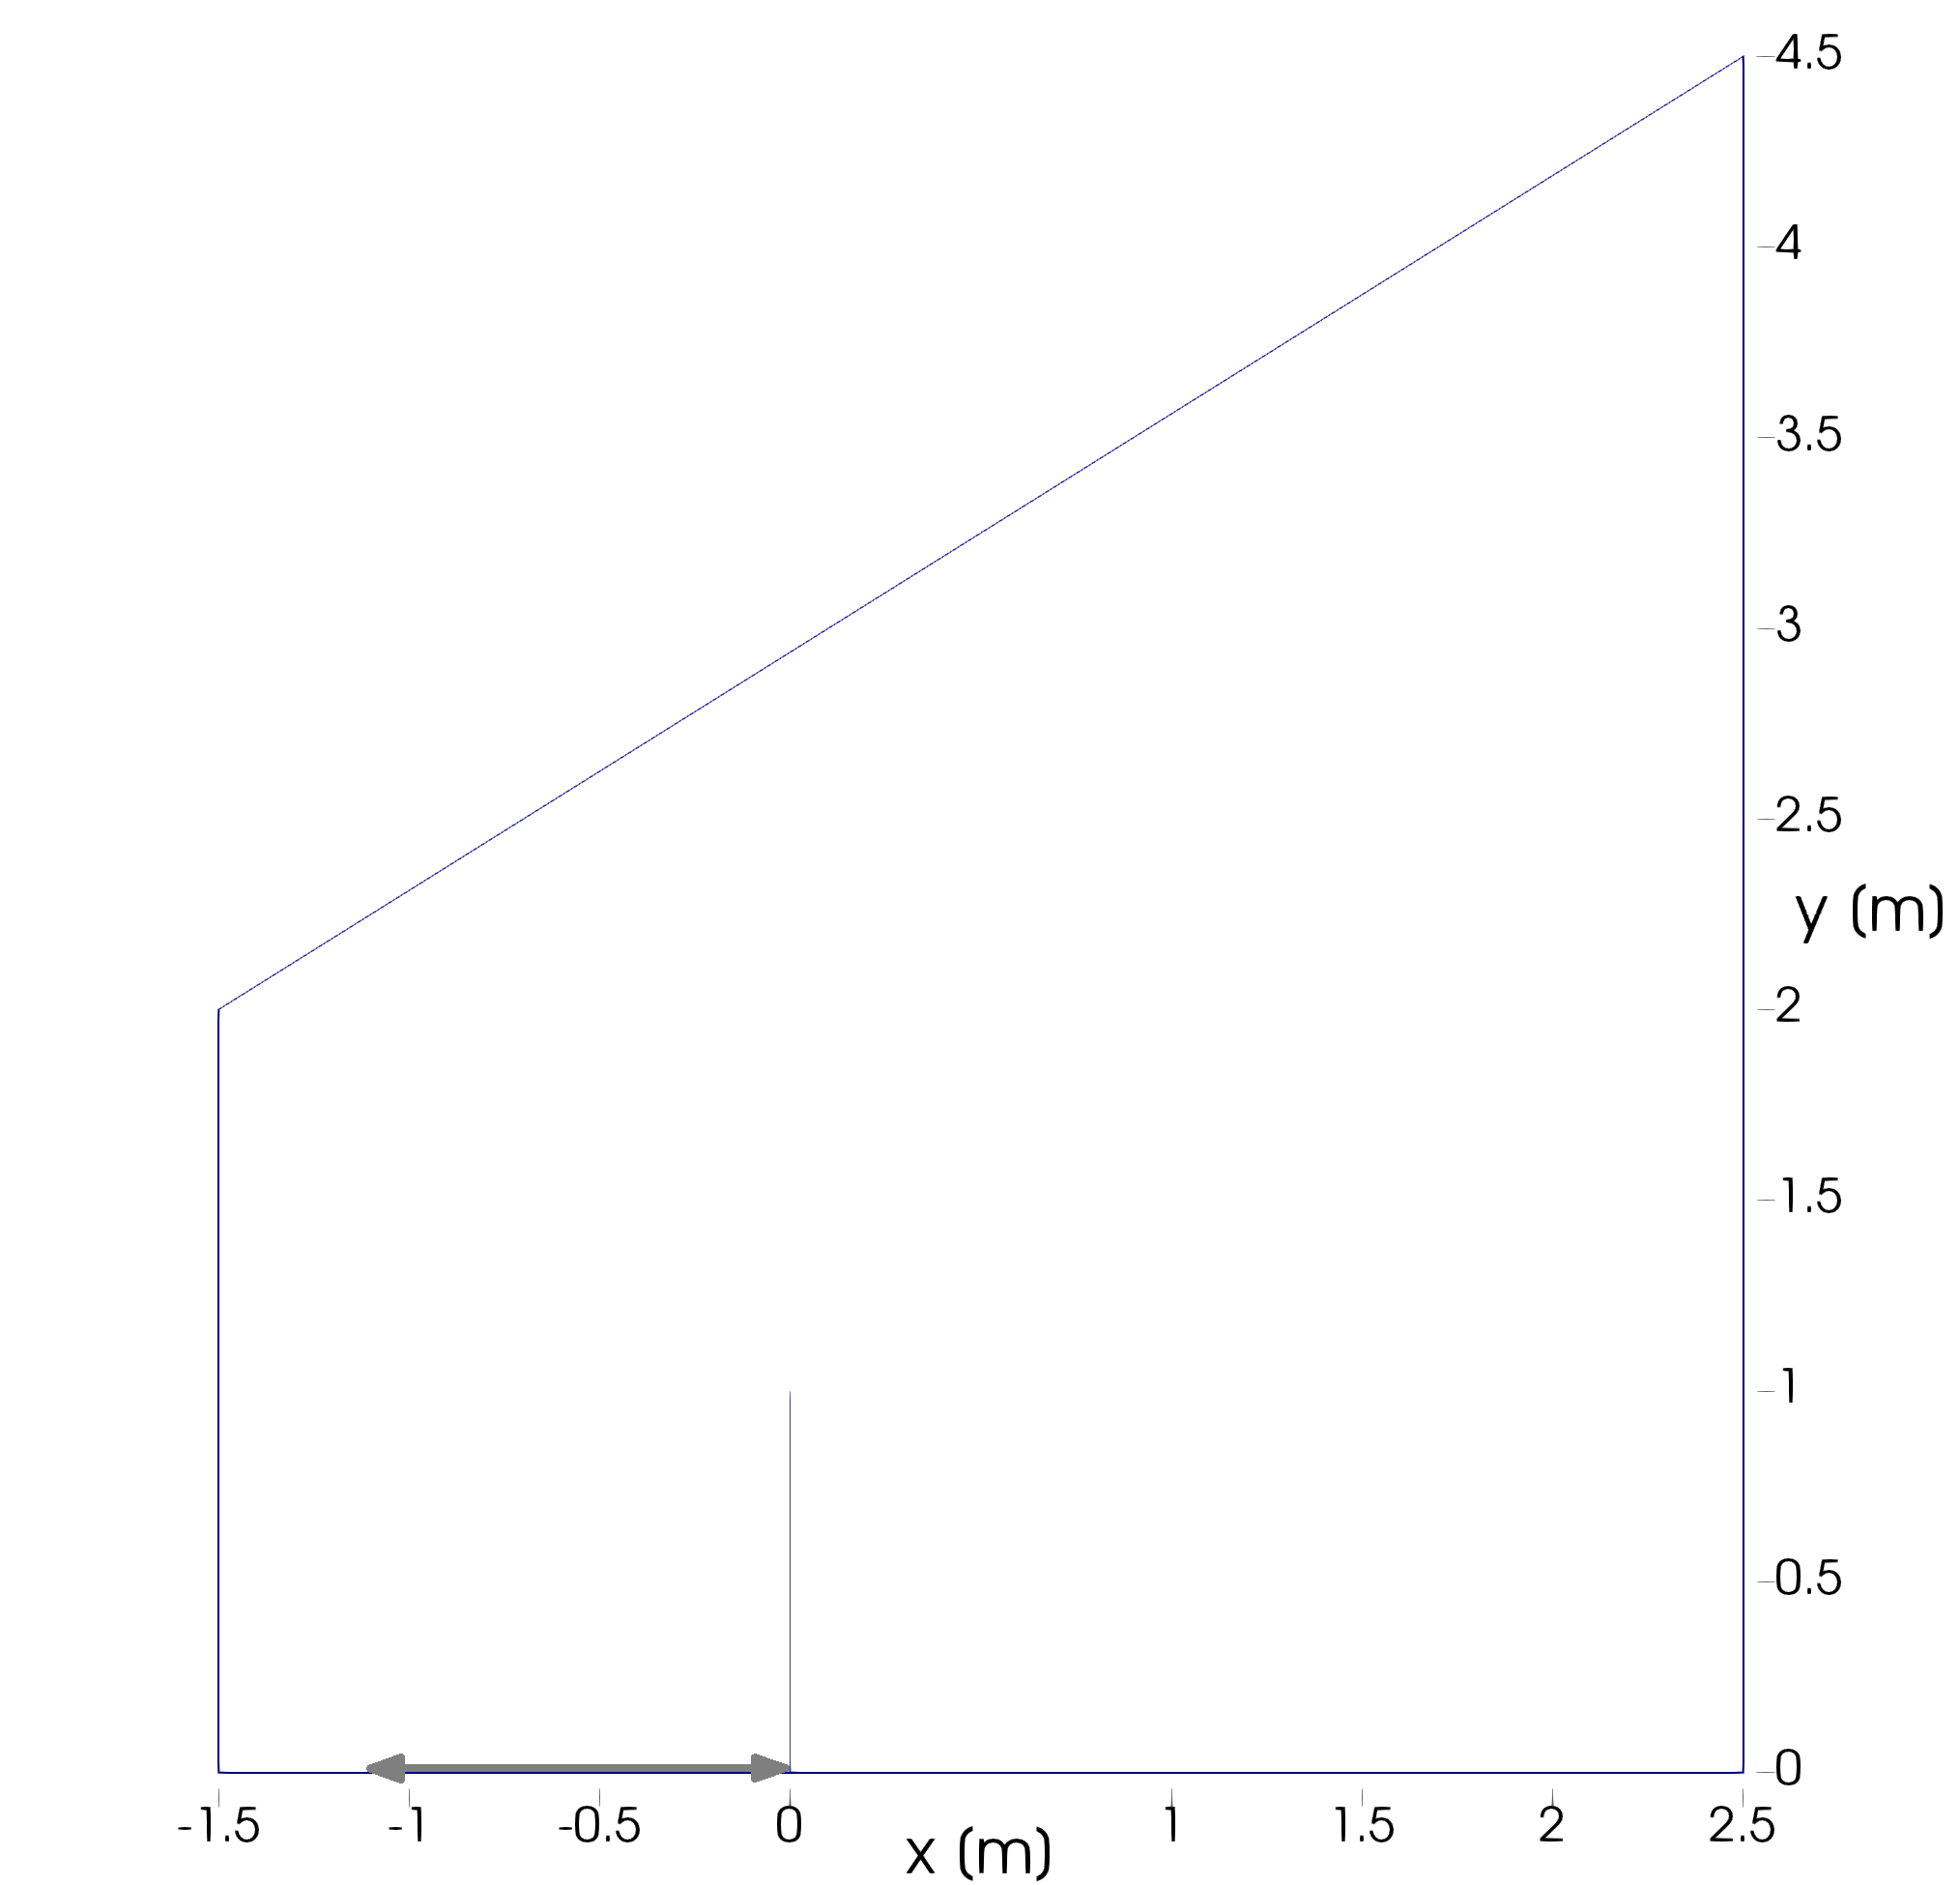
\includegraphics[width=0.6\textwidth] {./figures/line.png}
	            \caption{Stagnation line detail}
  \end{figure}
\end{frame}

\begin{frame}
  \frametitle{Temperature}
  \begin{figure}[ht]
    \centering
    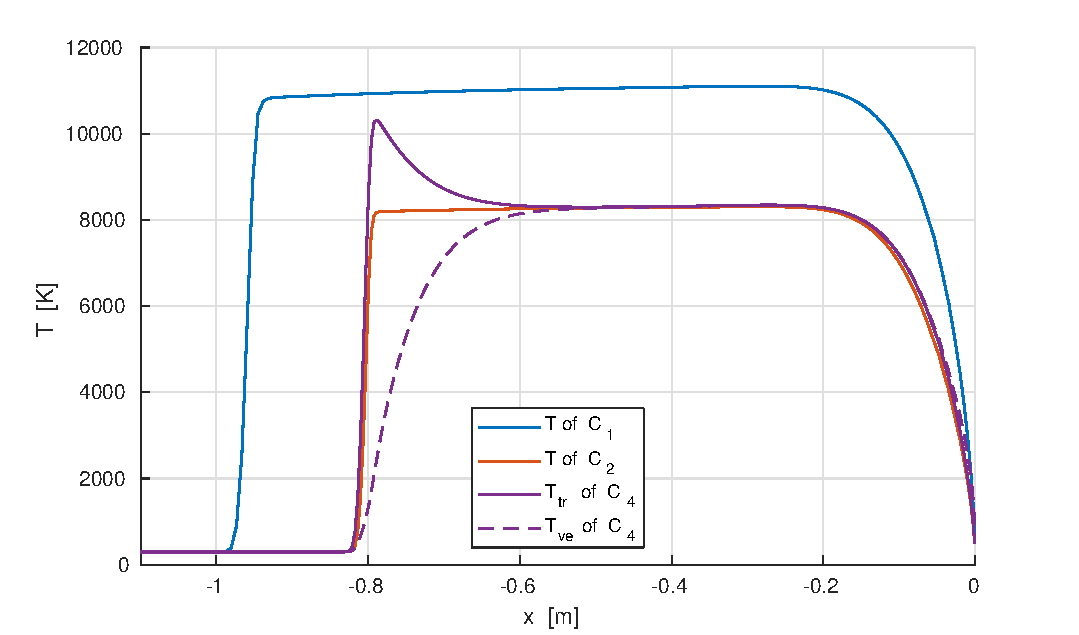
\includegraphics[width=\textwidth]{stagnationLine/figures/temperatureNReac.pdf}
    \caption{Non reacting test cases}
  \end{figure}
\end{frame}

\begin{frame}
  \begin{figure}[ht]
    \centering
    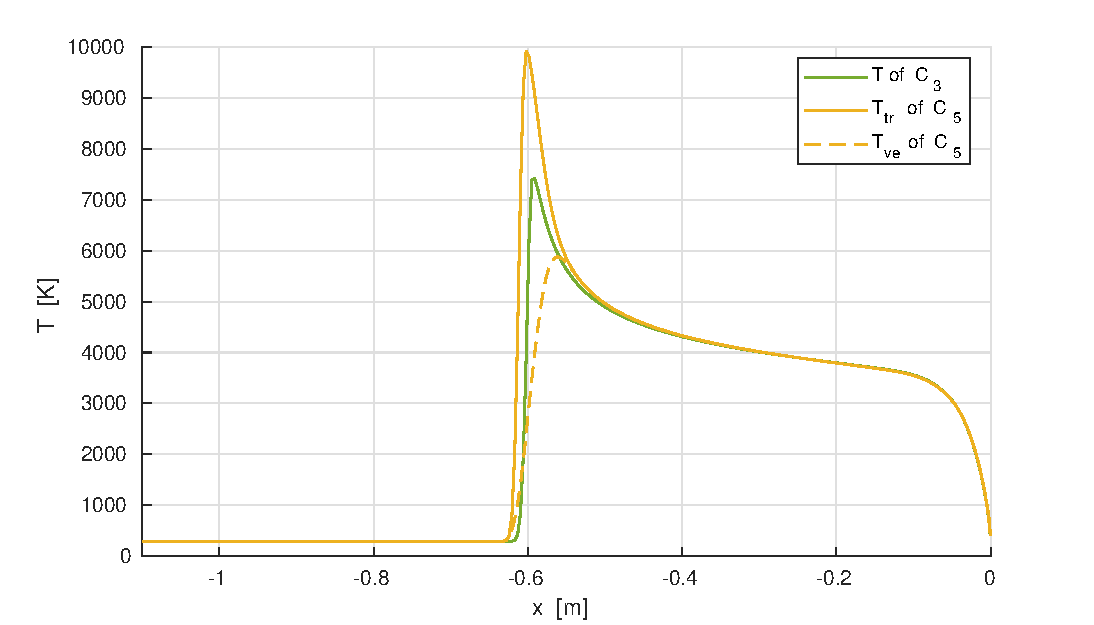
\includegraphics[width=\textwidth]{stagnationLine/figures/temperatureReac.pdf}
    \caption{Reacting test cases}
  \end{figure}
\end{frame}

\begin{frame}
  \frametitle{Nonequilibrium level} The level of nonequilibrium is measured by
  the following parameter
  \begin{equation*}
    \delta_{eq}=\frac{T_{tr}-T_{ve}}{T_{ve}}
  \end{equation*}
  \\ The extension of the nonequilibrium region, where $\delta_{eq}>0.01$, is
  also considered.
  \begin{table}[ht]
    \centering
    \caption{Nonequilibrium region length} \renewcommand{\arraystretch}{1.2}
    \setlength{\tabcolsep}{10pt}
    \begin{tabular}{ c c }
      \noalign{\hrule height 1pt} \textbf{Test Case} & \textbf{Value} [m]
      \bigstrut \\ \hline C$_4$ & 0.274092 \\ C$_5$ & 0.088750
      \\ \noalign{\hrule height 1pt}
    \end{tabular}
  \end{table}
\end{frame}

\begin{frame}
  \begin{figure}[ht]
    \centering
    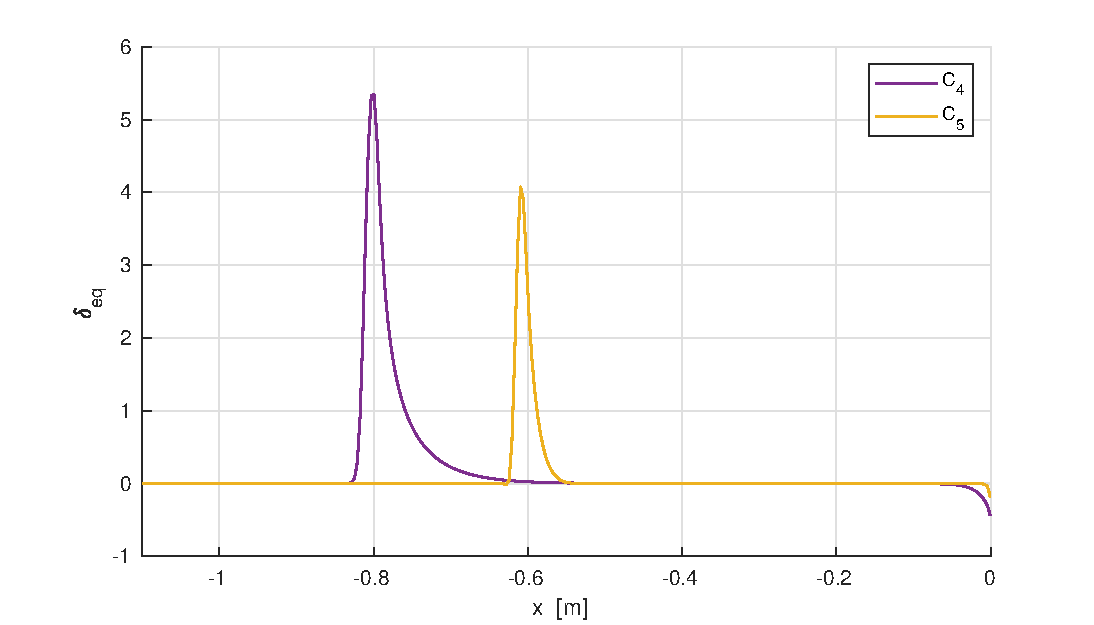
\includegraphics[width=\textwidth]{stagnationLine/figures/levelNoneq.pdf}
    \caption{Nonequilibrium test cases}
  \end{figure}
\end{frame}

\begin{frame}
  \frametitle{Specific Heat Capacities}
  \begin{figure}[ht]
    \centering
    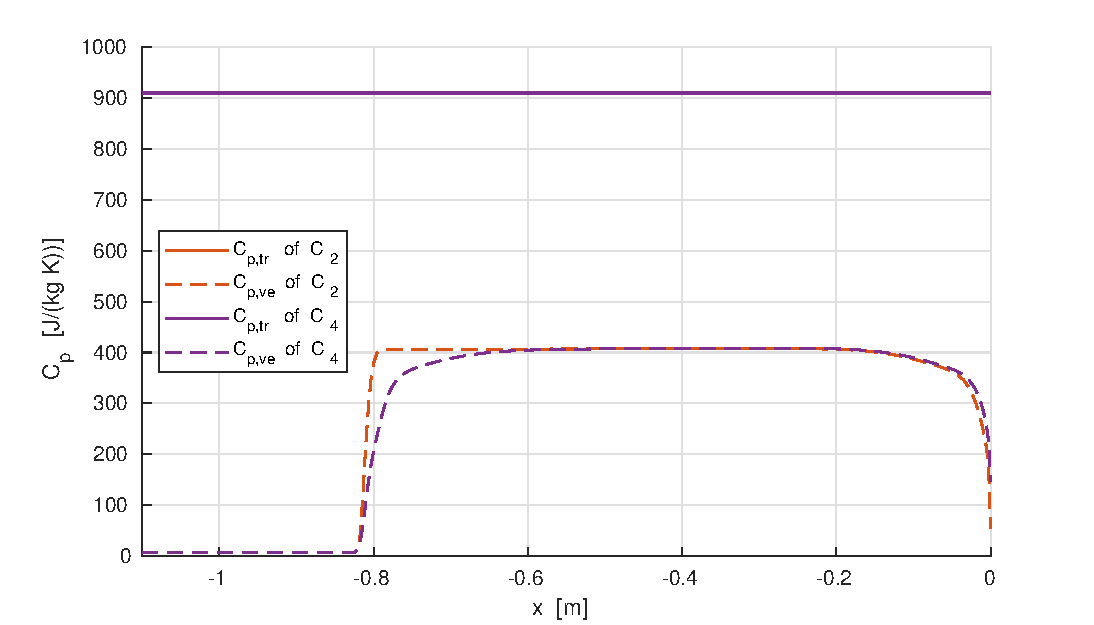
\includegraphics[width=\textwidth]{stagnationLine/figures/specificHeatNReac.pdf}
    \caption{Non reacting test cases}
  \end{figure}
\end{frame}

\begin{frame}
  \begin{figure}[ht]
    \centering
    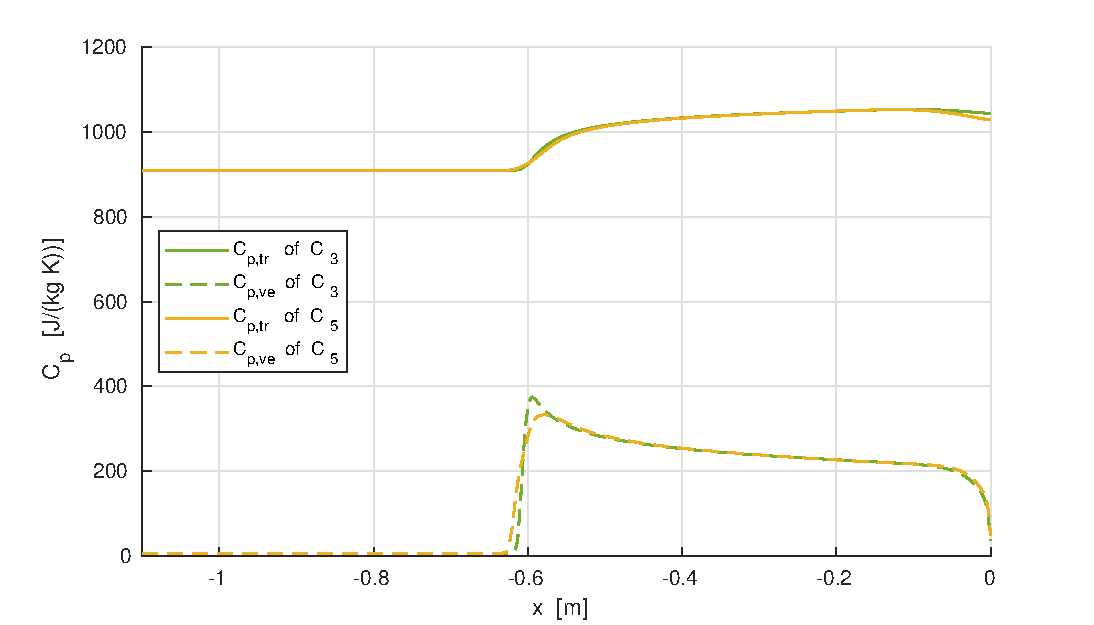
\includegraphics[width=\textwidth]{stagnationLine/figures/specificHeatReac.pdf}
    \caption{Reacting test cases}
  \end{figure}
\end{frame}

\begin{frame}
  \frametitle{Frozen Mach Number} In the calculation of this variable, the
  speed of sound, $a$, has been determined by
  \begin{equation*}
    a=\begin{cases} \sqrt{\bar{\gamma}RT_{tr}}&\text{for nonequilibrium cases}
    \\ \sqrt{\bar{\gamma}RT}&\text{for equilibrium cases}
    \end{cases}
  \end{equation*}
  where $\bar{\gamma}$ is defined to be the ratio of the frozen
  trans\-la\-tio\-nal-ro\-ta\-tio\-nal specific heats of the gas mixture
  \begin{equation*}
    \bar{\gamma}=\frac{C_{p,tr}}{C_{v,tr}}=1+\frac{R}{C_{v,tr}}=
    1+\frac{R}{\dfrac{5}{2}R}=\frac{7}{5}
  \end{equation*}
  The complete expression, which considers also the
  vi\-bra\-tio\-nal-elec\-tro\-nic specific heat, is not necessary since that
  the difference between the two formulations are very small.
\end{frame}

\begin{frame}
  \begin{figure}[ht]
    \centering
    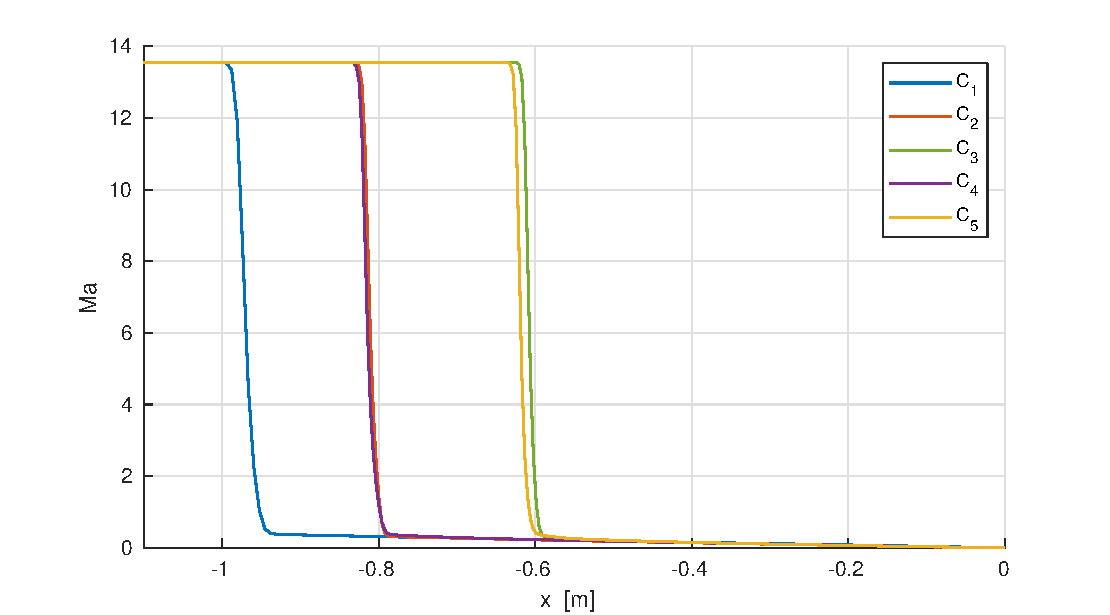
\includegraphics[width=\textwidth]{stagnationLine/figures/mach.pdf}
    \caption{Frozen mach number profiles}
  \end{figure}
\end{frame}

\begin{frame}
  \frametitle{Mixture Composition}
  \begin{figure}[ht]
    \centering
    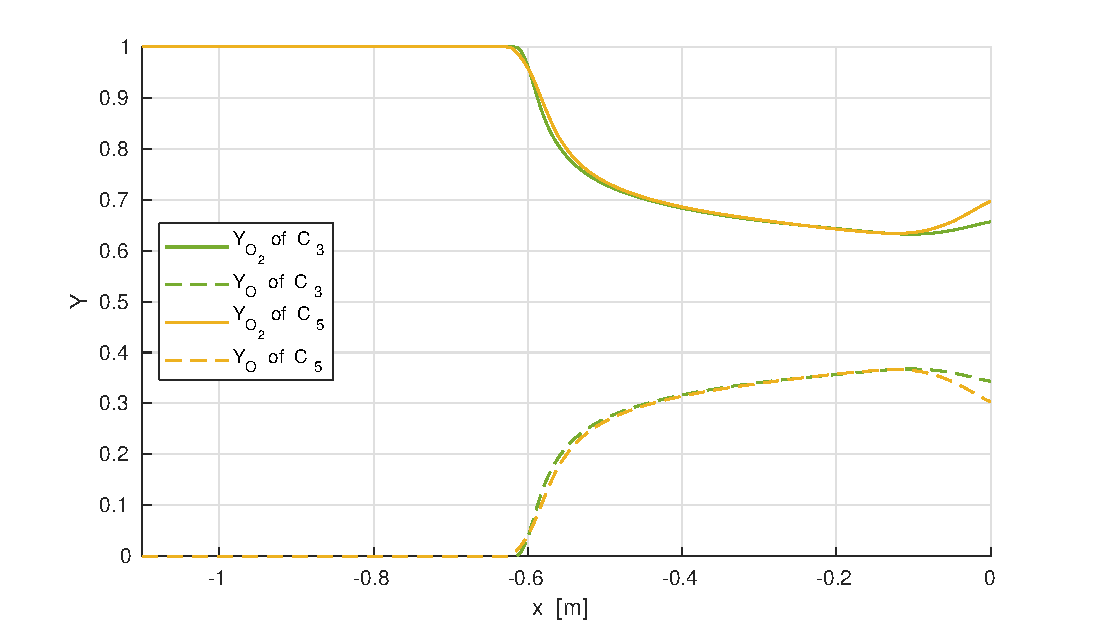
\includegraphics[width=\textwidth]{stagnationLine/figures/composition.pdf}
    \caption{Reacting test cases}
  \end{figure}
\end{frame}

\begin{frame}
  \frametitle{Number Density}
  \begin{figure}[ht]
    \centering
    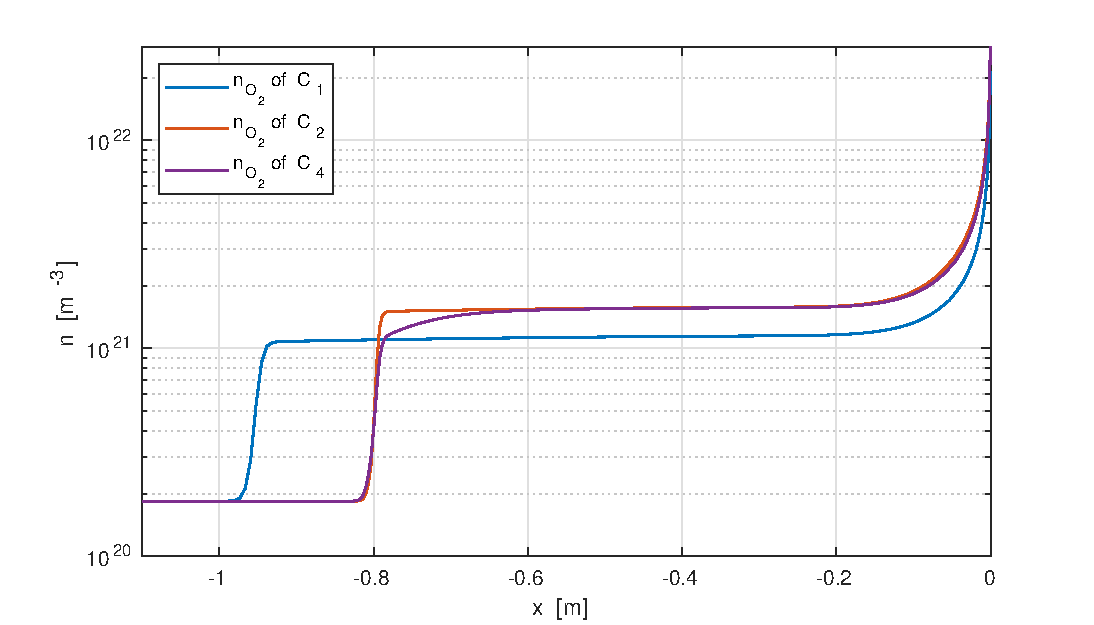
\includegraphics[width=\textwidth]{stagnationLine/figures/numbDenNReac.pdf}
    \caption{Non reacting test cases}
  \end{figure}
\end{frame}

\begin{frame}
  \begin{figure}[ht]
    \centering
    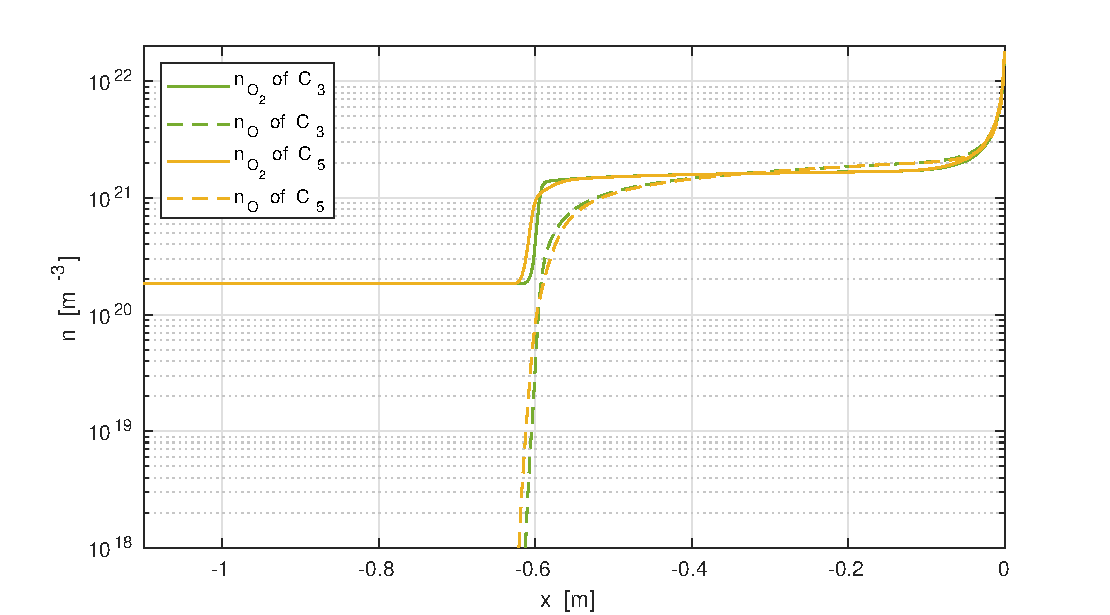
\includegraphics[width=\textwidth]{stagnationLine/figures/numbDenReac.pdf}
    \caption{Reacting test cases}
  \end{figure}
\end{frame}

\begin{frame}
  \frametitle{Pressure}
  \begin{figure}[ht]
    \centering
    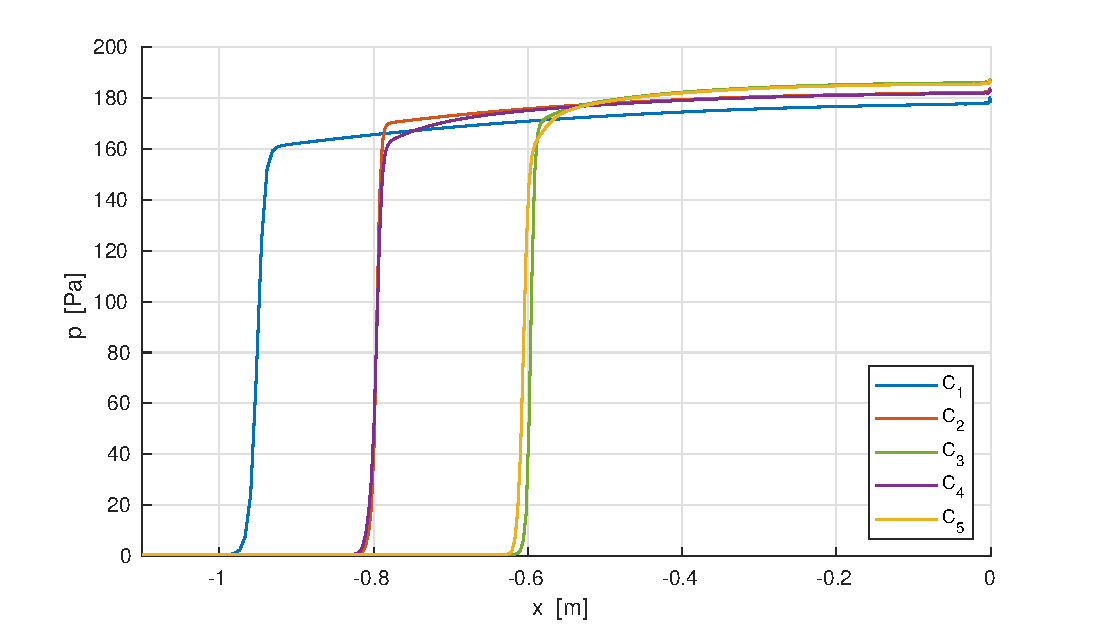
\includegraphics[width=\textwidth]{stagnationLine/figures/pressure.pdf}
  \end{figure}
\end{frame}

\begin{frame}
  \frametitle{Stand-off distance} The stand-off distance can be evaluated by
  considering the $x$-direction pressure gradient, $\partial{p}/\partial{x}$,
  whose maximum value position corresponds to the effective bow shock
  location.
  \begin{table}[ht]
    \centering
    \caption{Stand-off distance} \renewcommand{\arraystretch}{1.2}
    \setlength{\tabcolsep}{10pt}
    \begin{tabular}{ c c }
      \noalign{\hrule height 1pt} \textbf{Test Case} & \textbf{Value} [m]
      \bigstrut \\ \hline C$_1$ & 0.952280 \\ C$_2$ & 0.795787 \\ C$_3$ &
      0.594790 \\ C$_4$ & 0.795787 \\ C$_5$ & 0.605868 \\ \noalign{\hrule
        height 1pt}
    \end{tabular}
  \end{table}
\end{frame}

\begin{frame}
  \begin{figure}[ht]
    \centering 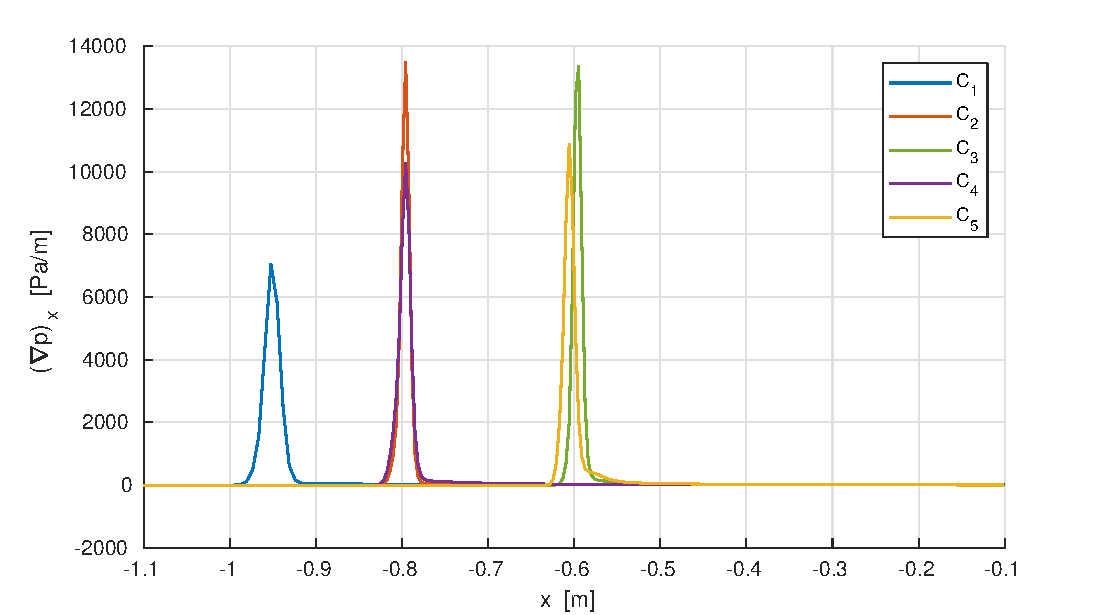
\includegraphics[width=\textwidth]
               {stagnationLine/figures/standOff.pdf}
	            \caption{$x$-direction pressure gradient,
                      $\partial{p}/\partial{x}$, profiles}
  \end{figure}
\end{frame}


\section{Surface Quantities}

\begin{frame}
  In this section fundamental surface properties are analyzed over the
  $y$-dimensional baffle wall, in particular the only face exposed to the
  incoming wind.
  \begin{figure}[H]
    \centering 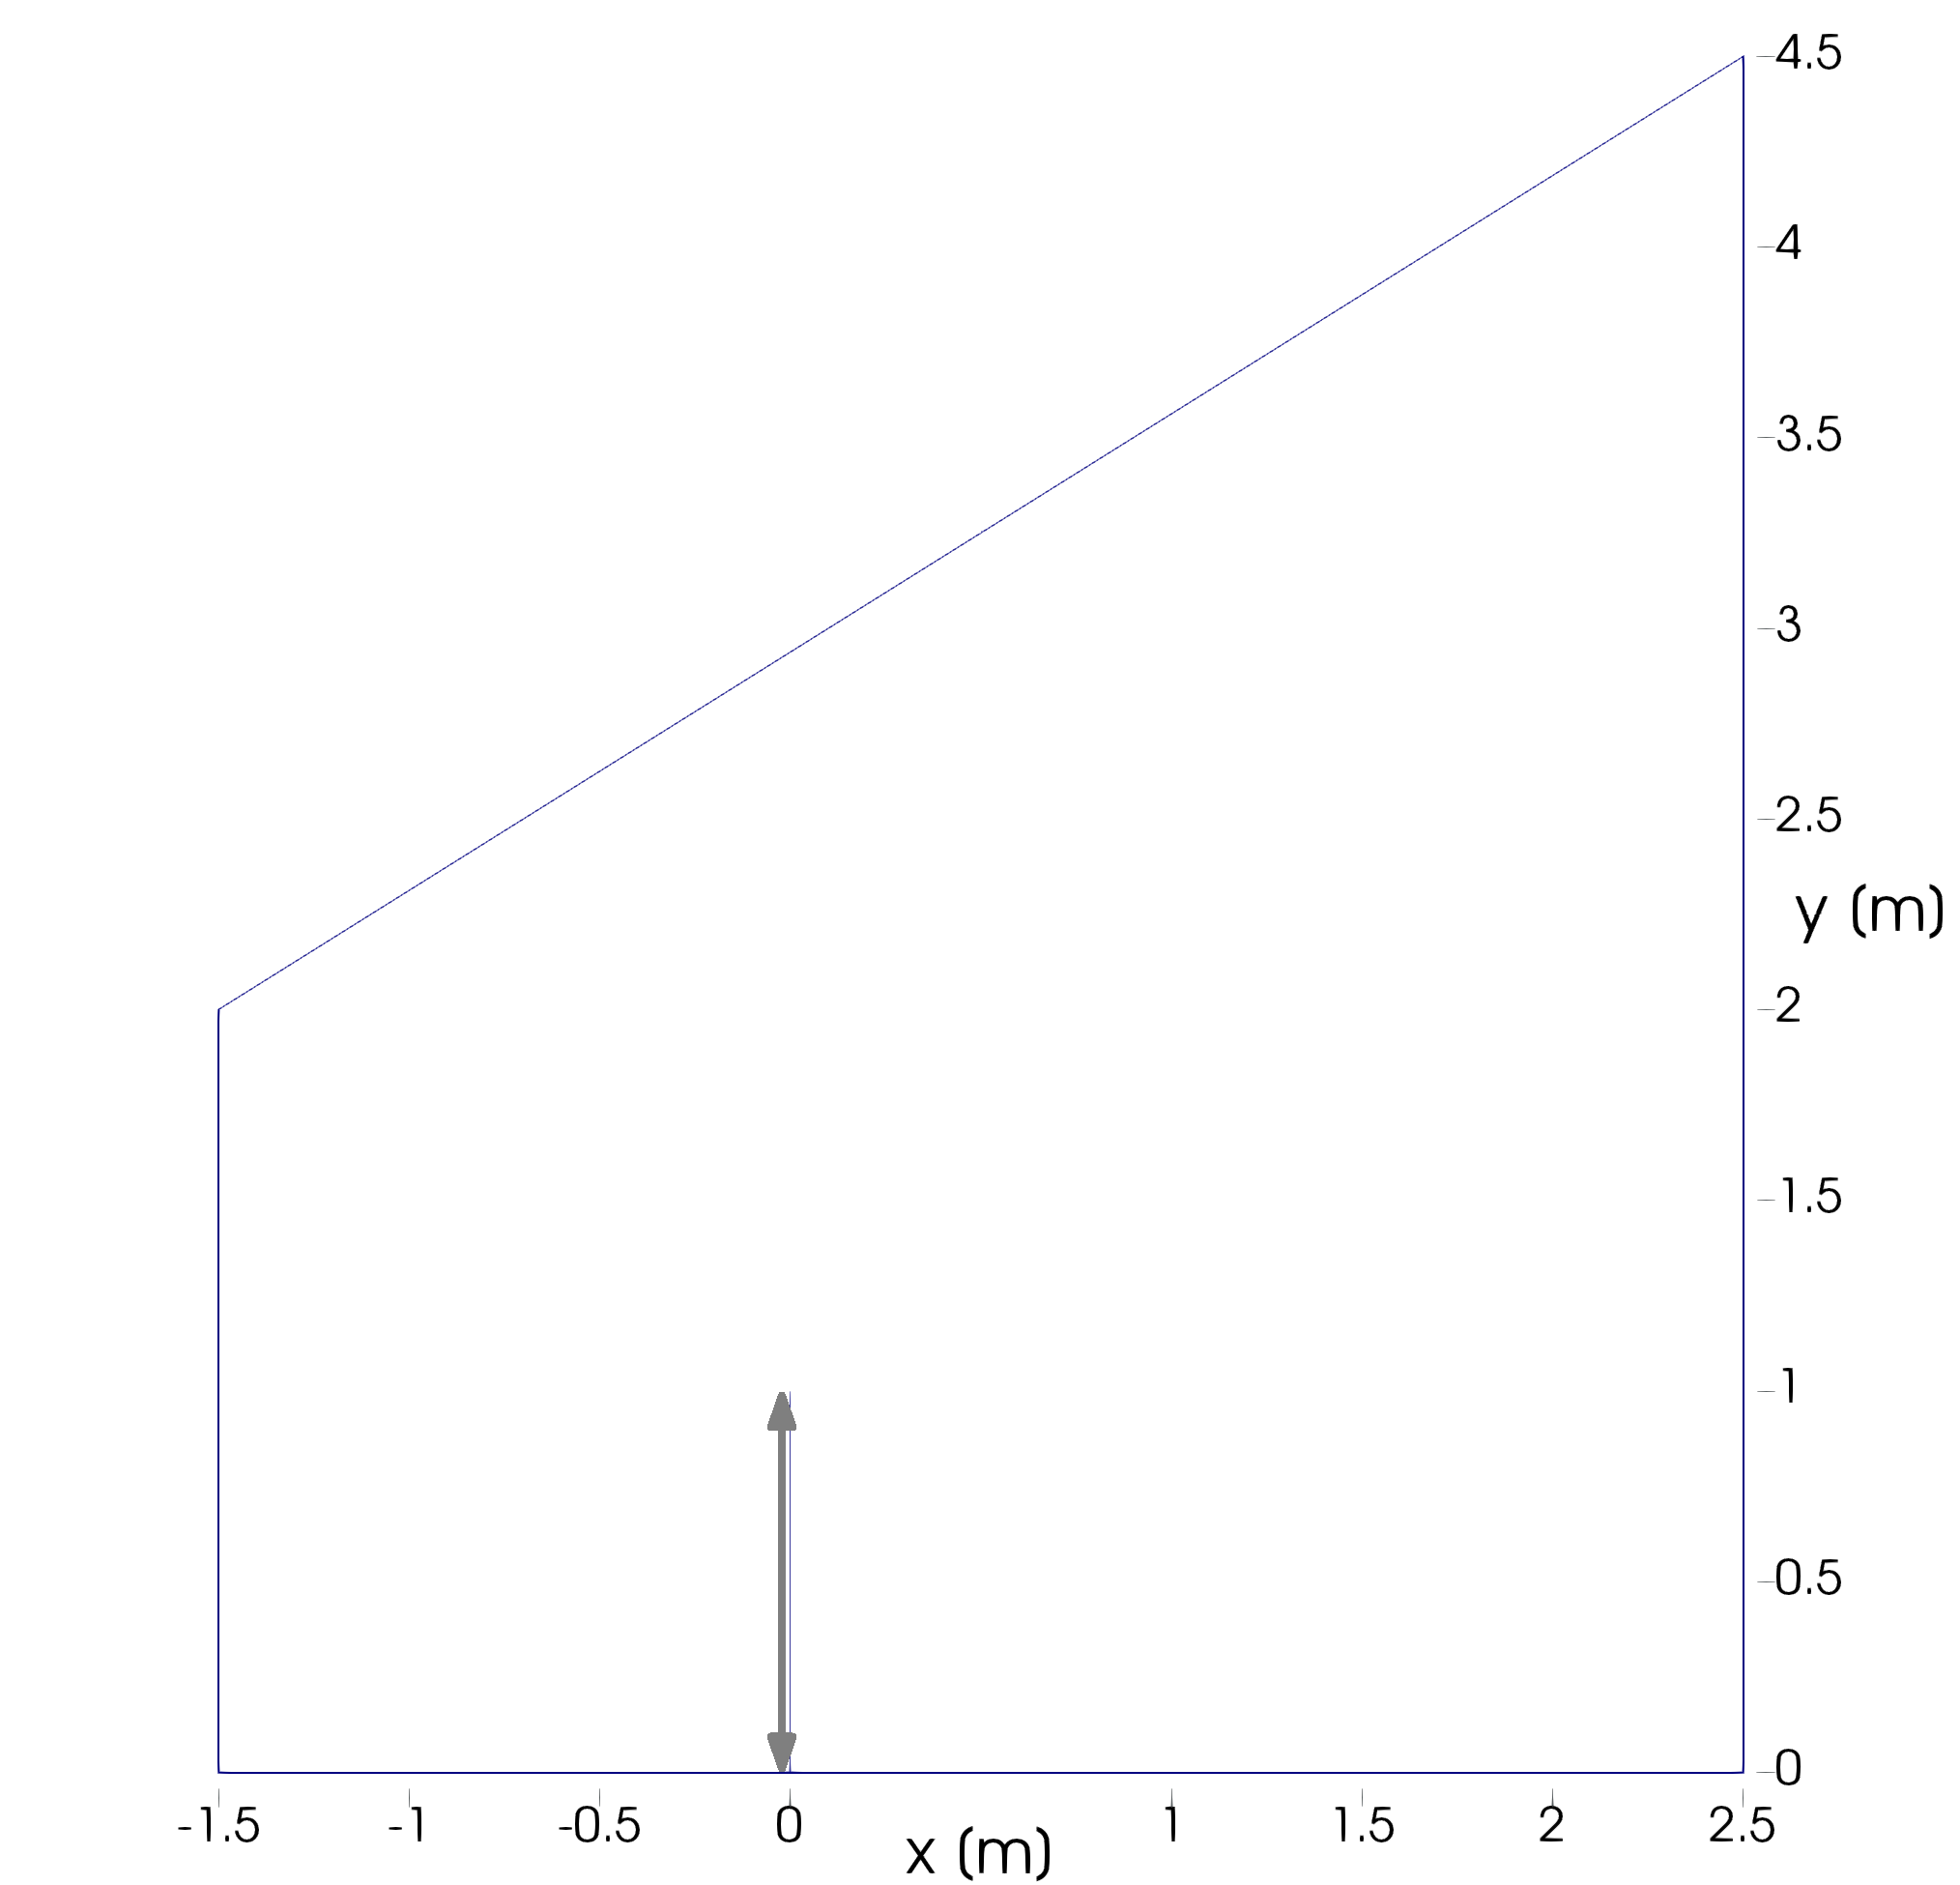
\includegraphics[width=0.6\textwidth] {./figures/surface.png}
	            \caption{Baffle face analyzed}
	            \label{fig:surface}
  \end{figure}
\end{frame}

\begin{frame}
  \frametitle{Friction Coefficient} The friction coefficient, $C_f$, is given
  by
  \begin{equation*}
    C_f=\frac{\tau_w}{\dfrac{1}{2}\rho_\infty u_\infty^2}
  \end{equation*}
  where $\tau_w$ is the local wall shear stress defined by
  \begin{equation*}
    \tau_w=|\left(\boldsymbol{\tau}\right)_w\cdot
    \left(\textbf{I}-\boldsymbol{nn}\right)|
  \end{equation*}
  \vspace{-7mm}
  \begin{table}[ht]
    \centering
    \caption{$C_f$ values at 0.9 m high} \renewcommand{\arraystretch}{1.2}
    \setlength{\tabcolsep}{10pt}
    \begin{tabular}{ c c }
      \noalign{\hrule height 1pt} \textbf{Test Case} & \textbf{Value}
      \bigstrut \\ \hline C$_1$ & 0.0401197 \\ C$_2$ & 0.0264864 \\ C$_3$ &
      0.0241662 \\ C$_4$ & 0.0289175 \\ C$_5$ & 0.0252766 \\ \noalign{\hrule
        height 1pt}
    \end{tabular}
  \end{table}
\end{frame}

\begin{frame}
  \begin{figure}[ht]
    \centering 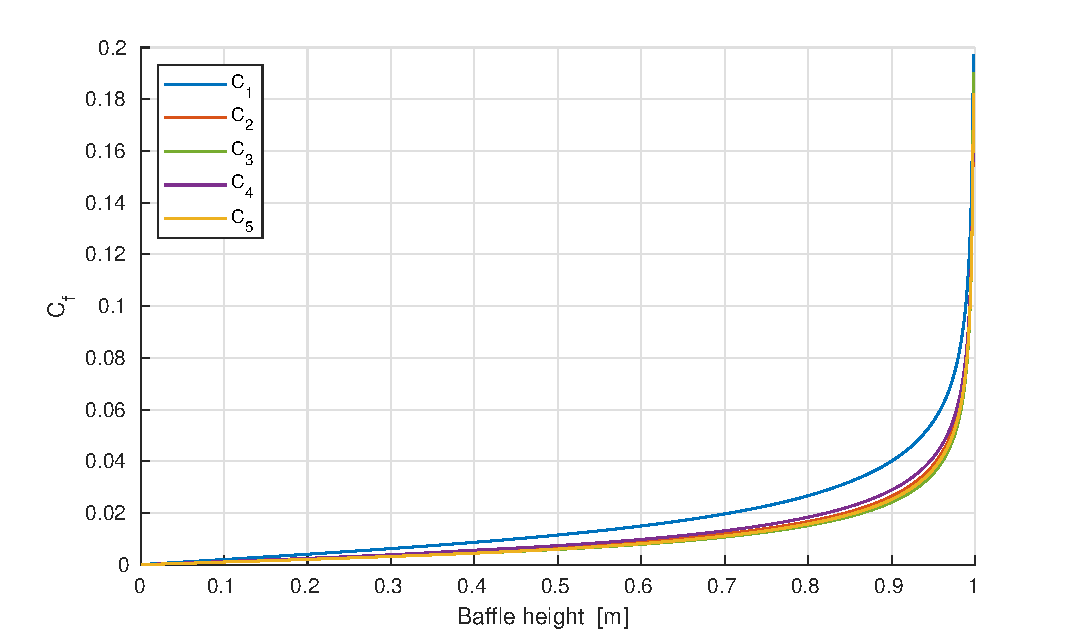
\includegraphics[width=\textwidth]
               {obstacleSurface/figures/Friction.pdf}
	            \caption{Friction coefficient evolution over the baffle
                      wall}
  \end{figure}
\end{frame}

\begin{frame}
  \frametitle{Stanton Number} The Stanton number, $St$, is given by
  \begin{equation*}
    St=\frac{\boldsymbol{n}\cdot\left(\boldsymbol{q}\right)_w}
    {\dfrac{1}{2}\rho_\infty u_\infty^3}
  \end{equation*}
  where $\left(\boldsymbol{q}\right)_w$ is the wall heat flux, for which
  vector $\boldsymbol{q}$ can be expressed by
  \begin{equation*}
    \boldsymbol{q}=\boldsymbol{q}_{tr}+\boldsymbol{q}_{ve}
  \end{equation*}
  \vspace{-7mm}
  \begin{table}[ht]
    \centering
    \caption{$St$ values at 0.9 m high} \renewcommand{\arraystretch}{1.2}
    \setlength{\tabcolsep}{10pt}
    \begin{tabular}{ c c }
      \noalign{\hrule height 1pt} \textbf{Test Case} & \textbf{Value}
      \bigstrut \\ \hline C$_1$ & 0.0728805 \\ C$_2$ & 0.0509591 \\ C$_3$ &
      0.0194913 \\ C$_4$ & 0.0570390 \\ C$_5$ & 0.0201023 \\ \noalign{\hrule
        height 1pt}
    \end{tabular}
  \end{table}
\end{frame}

\begin{frame}
  \begin{figure}[ht]
    \centering 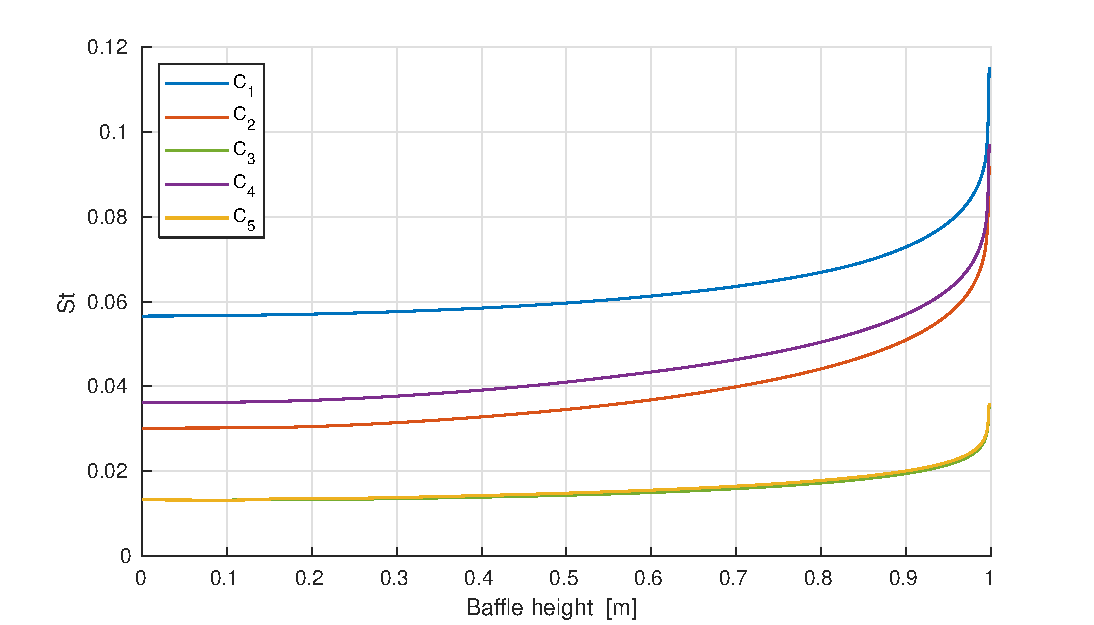
\includegraphics[width=\textwidth]
               {obstacleSurface/figures/Stanton.pdf}
                    \caption{Stanton number evolution over the baffle wall}
  \end{figure}
\end{frame}


\section{A\-ero\-thermo\-dyna\-mic Coefficients}

\begin{frame}
  \frametitle{Drag Coefficient} It can be simply expressed by
  \begin{equation*}
    C_{\scalebox{0.6}{\textit{D}}}=\frac{D} {\dfrac{1}{2}\rho_\infty
      u_\infty^2A_{ref}}
  \end{equation*}
  \begin{table}[ht]
    \centering
    \caption{$C_{\scalebox{0.6}{\textit{D}}}$ values}
    \renewcommand{\arraystretch}{1.2} \setlength{\tabcolsep}{10pt}
    \begin{tabular}{ c c }
      \noalign{\hrule height 1pt} \textbf{Test Case} & \textbf{Value}
      \bigstrut \\ \hline C$_1$ & 0.7627369 \\ C$_2$ & 0.7870324 \\ C$_3$ &
      0.8160124 \\ C$_4$ & 0.7876704 \\ C$_5$ & 0.8387780 \\ \noalign{\hrule
        height 1pt}
    \end{tabular}
  \end{table}
\end{frame}

\begin{frame}
  \frametitle{Integrated Heat Flux} It can be simply expressed by
  \begin{equation*}
    C_{\scalebox{0.6}{\textit{H}}}=\int_{S_w}\left(\boldsymbol{q}\right)_w\cdot
    d\boldsymbol{S}=\int_{S_w}\left(\boldsymbol{q}\right)_w\cdot\boldsymbol{n}dS
  \end{equation*}
  \begin{table}[ht]
    \centering
    \caption{$C_{\scalebox{0.6}{\textit{H}}}$ values}
    \renewcommand{\arraystretch}{1.2} \setlength{\tabcolsep}{5pt}
    \begin{tabular}{ *{4}{c} }
      \noalign{\hrule height 1pt} \textbf{Test Case} & \textbf{Value} [W] &
      \textbf{\% trans-rot.} & \textbf{\% vibro-elec.} \bigstrut \\ \hline
      C$_1$ & 267.646 & 100 & 0 \\ C$_2$ & 162.205 & 97.7048 &
      \phantom{1}2.2952 \\ C$_3$ & \phantom{1}66.381 & 98.3786 &
      \phantom{1}1.6214 \\ C$_4$ & 188.862 & 79.4157 & 20.5843 \\ C$_5$ &
      \phantom{1}68.087 & 96.0405 & \phantom{1}3.9595 \\ \noalign{\hrule
        height 1pt}
    \end{tabular}
  \end{table}
\end{frame}

\end{document}
